\documentclass[conference]{IEEEtran}
\IEEEoverridecommandlockouts
\usepackage{cite}
\usepackage{amsmath,amssymb}
\usepackage{graphicx}
\usepackage{tikz}
\usetikzlibrary{positioning,arrows.meta,shapes.geometric}
\usepackage{booktabs}
\usepackage{url}
\usepackage[hidelinks]{hyperref}
\usepackage{textcomp}
\def\BibTeX{{\rm B\kern-.05em{\sc i\kern-.025em b}\kern-.08em T\kern-.1667em\lower.7ex\hbox{E}\kern-.125em X}}

\begin{document}

\title{CollabDoc: A Real-Time Collaborative Document Editor with Operational Transformation and Stylometric Authorship Attribution}

\author{\IEEEauthorblockN{Nitish Kumar}
\IEEEauthorblockA{\textit{{[Department], [Institution]}}\\
{[City, Country]}\\
nitish@admrls.com}
\and
\IEEEauthorblockN{Balan N}
\IEEEauthorblockA{\textit{{[Department], [Institution]}}\\
{[City, Country]}\\
{[email]}}
}

\maketitle

\begin{abstract}
Group documents are routinely written by several people at once, yet the tools that let them edit together say little about who actually wrote what. This paper presents CollabDoc, a real-time collaborative document editor that couples a server-arbitrated operational transformation (OT) engine with an authorship-attribution engine. Edits converge under arbitrary concurrency; a run-length keystroke ledger records mechanical authorship; and a dependency-free softmax classifier over 44 scale-free stylometric features forms an independent opinion about the style of each block. The two sources of evidence are blended with a weight that depends on how much text a block offers, and a leave-one-out check flags passages that were typed by one collaborator but read like another's writing. The system runs as a single process or as a Kubernetes deployment in which a document-aware router pins each document to one pod and a Kafka broadcaster carries presence and notifications between pods. On a development machine the server acknowledged edits with a 2.3\,ms median and 3.9\,ms 95th-percentile round trip, against a 200\,ms requirement; the OT engine converged on 2000 randomised concurrent-edit pairs; and the browser port of the engine agreed with the server implementation on every randomly generated case. We also describe the engineering decisions that shaped the design, including a teardown bug that silently dropped the last second of typing.
\end{abstract}

\begin{IEEEkeywords}
operational transformation, collaborative editing, authorship attribution, stylometry, keystroke dynamics, WebSocket, Kafka, Kubernetes
\end{IEEEkeywords}

%--------------------------------------------------------------------
\section{Introduction}
Real-time co-editing has moved from research prototypes~\cite{ellis1989,nichols1995} to an everyday tool. Its central difficulty is unchanged: when two users edit the same text concurrently, every replica must end in the same state without discarding either user's intention~\cite{sun1998}. Two families of algorithms address this. Operational transformation (OT) rewrites each incoming operation against the operations that landed concurrently~\cite{ellis1989,sun1998,sun1998ot}; conflict-free replicated data types (CRDTs) design the data structure so that merges commute~\cite{shapiro2011,roh2011,weiss2009,nicolaescu2016}.

Convergence is only half of what a group of authors needs. In coursework, research teams and editorial settings, the question that follows a shared draft is \emph{who wrote this?} Authorship attribution has a long computational history~\cite{mosteller1963,stamatatos2009,koppel2009,juola2006}, but it is normally applied to finished text and independently of the editor that produced it. A collaborative editor, however, observes something a stylometric model never sees: every keystroke and its owner.

CollabDoc combines the two. The editing core gives the system an authoritative, append-only operation log; the attribution engine uses that log both as evidence and as the source of training labels. The remainder of this paper states the problem, describes the architecture, and reports measurements taken from the implementation.

%--------------------------------------------------------------------
\section{Problem Statement}
We target a document server that satisfies the following requirements, derived from the project's software requirements specification (SRS):
\begin{enumerate}
\item \textbf{Convergence.} Any interleaving of concurrent edits leaves all clients and the server holding identical text.
\item \textbf{Latency.} A real-time update is acknowledged and fanned out within 200\,ms.
\item \textbf{Attribution.} Each block of text is assigned to a collaborator with a calibrated confidence, and the system declines to answer when it lacks evidence.
\item \textbf{History.} Every version can be reconstructed and rolled back without rewriting the log.
\item \textbf{Scale-out.} The service runs on several backends without corrupting a document's state.
\item \textbf{Security.} Role-based access, safe rendering, and no disclosure of whether a document exists to a caller without access.
\end{enumerate}

%--------------------------------------------------------------------
\section{Highlights and Novelty}
\begin{itemize}
\item \textbf{Ledger-supervised stylometry.} Text that the keystroke ledger proves a user typed becomes that user's labelled corpus, so the classifier learns from the mechanical record and then forms an opinion independent of it.
\item \textbf{Length-aware blending.} Stylometric weight $\min(1,\ell/\ell_{0})$ scaled by a $0.65$ cap, so a four-word heading is decided by keystrokes and a full paragraph mostly by style, and the model can never fully overrule the recorded keystrokes.
\item \textbf{Leave-one-out integrity report.} A passage is judged by a model retrained \emph{without} it, removing the self-vouching effect of copied text; the report also lists pastes and per-person effort.
\item \textbf{Honest abstention.} With fewer than two authors with three samples each, the model returns ``not trained'' and attribution falls back to the ledger.
\item \textbf{Dependency-free classifier.} About 200 lines of softmax regression; a fitted model is a few hundred floats and trains in milliseconds, so attribution runs inline rather than behind a model-serving hop.
\item \textbf{Dual OT implementations, cross-checked.} Server (Python) and browser (JavaScript) engines are compared on random edits.
\item \textbf{Single code path for scale-out.} All events leave through a broadcaster interface even in one process; a document-aware router keeps each document on one pod.
\end{itemize}

%--------------------------------------------------------------------
\section{Related Work}
\subsection{Collaborative editing}
Ellis and Gibbs introduced dOPT and the idea of transforming concurrent operations~\cite{ellis1989}. The Jupiter system simplified the problem by routing all operations through a central server, so each client only needs to transform against one peer~\cite{nichols1995}; CollabDoc follows this server-centric model. Ressel et al.~\cite{ressel1996} and Sun et al.~\cite{sun1998} formalised the convergence, causality and intention-preservation goals, and Sun and Ellis surveyed the algorithms~\cite{sun1998ot}. Oster et al.\ showed that several early transformation functions violate convergence and proposed the TTF approach~\cite{oster2006}. CRDTs~\cite{shapiro2011} include Logoot~\cite{weiss2009}, RGA~\cite{roh2011}, a JSON datatype~\cite{kleppmann2017} and the Yjs framework~\cite{nicolaescu2016}; Attiya et al.\ give a specification and complexity bounds for collaborative text editing~\cite{attiya2016}. Differential synchronization~\cite{fraser2009} takes a diff-and-patch approach, and local-first software~\cite{kleppmann2019} motivates offline-capable designs. We chose OT because the system already has an authoritative server and because the operation log doubles as the version history.

\subsection{Authorship attribution}
Mosteller and Wallace's study of the \emph{Federalist Papers} established function-word frequencies as stylistic evidence~\cite{mosteller1963}. Surveys by Juola~\cite{juola2006}, Koppel et al.~\cite{koppel2009} and Stamatatos~\cite{stamatatos2009} organise later work, Burrows' Delta~\cite{burrows2002,evert2017} remains a strong baseline, and Narayanan et al.\ examine attribution at internet scale~\cite{narayanan2012}.

\subsection{Keystroke dynamics}
Keystroke timing is a well-studied biometric for authentication~\cite{monrose2000,killourhy2009,banerjee2012}. CollabDoc uses keystrokes differently: not their timing, but their \emph{ownership} within a shared buffer.

%--------------------------------------------------------------------
\section{System Architecture}
Fig.~\ref{fig:arch} shows the request paths. REST handles everything that is not a keystroke (accounts, documents, sharing, history); a WebSocket~\cite{rfc6455} carries editing, presence and attribution updates. Both read through a per-document \texttt{DocumentSession}, so a REST read during an edit returns the live text. The server is FastAPI~\cite{fastapi} with SQLAlchemy over SQLite or PostgreSQL; the client is plain JavaScript with no build step.

\begin{figure}[t]
\centering
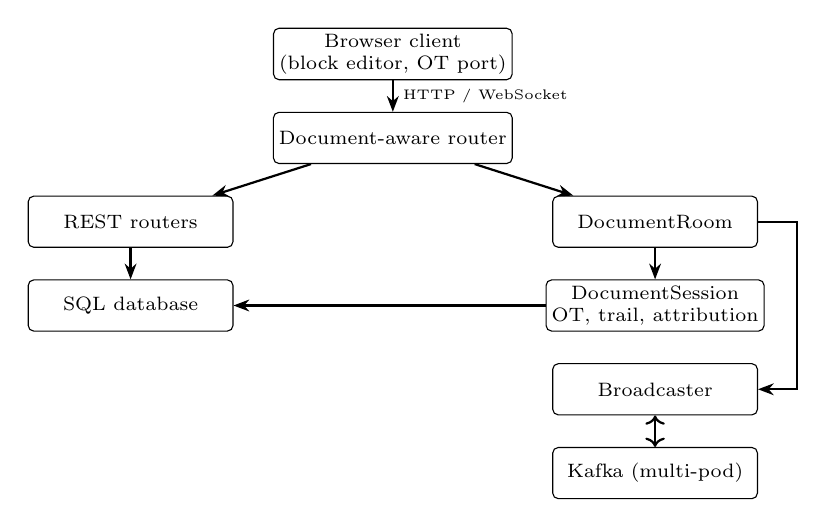
\begin{tikzpicture}[
  node distance=4mm,
  box/.style={draw,rounded corners=2pt,minimum height=6.5mm,minimum width=2.6cm,align=center,font=\scriptsize,inner sep=2pt},
  arr/.style={-{Stealth[length=2mm]},thick}]
\node[box] (cl) {Browser client\\(block editor, OT port)};
\node[box,below=of cl] (rt) {Document-aware router};
\node[box,below left=4mm and -3mm of rt,xshift=-8mm] (rest) {REST routers};
\node[box,below right=4mm and -3mm of rt,xshift=8mm] (room) {DocumentRoom};
\node[box,below=of room] (ses) {DocumentSession\\OT, trail, attribution};
\node[box,below=of rest] (db) {SQL database};
\node[box,below=of ses] (bc) {Broadcaster};
\node[box,below=of bc] (kf) {Kafka (multi-pod)};
\draw[arr] (cl) -- node[right,font=\tiny]{HTTP / WebSocket} (rt);
\draw[arr] (rt) -- (rest);
\draw[arr] (rt) -- (room);
\draw[arr] (rest) -- (db);
\draw[arr] (room) -- (ses);
\draw[arr] (ses) -- (db);
\draw[arr] (room.east) -- ++(5mm,0) |- (bc.east);
\draw[arr,<->] (bc) -- (kf);
\end{tikzpicture}
\caption{Request paths. Every event, even in a single process, leaves through the broadcaster and returns through a subscription.}
\label{fig:arch}
\end{figure}

\subsection{Data model}
Seven tables map the hybrid model of the SRS through one ORM: users, documents, collaborators (OWNER/EDITOR/VIEWER), the operation log (one row per accepted operation), parsed blocks with attribution, periodic snapshots, and author samples. Block order uses a lexical rank, so concurrent inserts never renumber their neighbours. A rollback appends the inverse of the interval rather than rewriting history, so the log stays append-only and auditable.

%--------------------------------------------------------------------
\section{Operational Transformation Engine}
An operation is a sequence of \emph{retain}, \emph{insert} and \emph{delete} components over a plain-text buffer, serialised as a flat JSON array such as \texttt{[5, -2, "hi", 9]}. Builders keep operations canonical: adjacent retains merge, and an insert precedes a delete at the same position. Transformation must satisfy the convergence property
\begin{equation}
(a',b')=T(a,b)\;\Rightarrow\;
\mathrm{ap}(\mathrm{ap}(d,a),b')=\mathrm{ap}(\mathrm{ap}(d,b),a'),
\label{eq:tp1}
\end{equation}
where $\mathrm{ap}$ applies an operation to a document $d$. Concurrent inserts at the same offset are tie-broken in favour of the first argument, so all replicas resolve ties identically.

\textbf{Server rebasing.} The server holds the text, a version counter and the operation log. A client sends \texttt{\{version, operation\}}; the server transforms it against every logged operation after that version, applies it, appends it, and broadcasts the transformed form. The sender receives an acknowledgement rather than an echo, which lets the client run the standard three-state machine (synchronised, awaiting confirmation, awaiting with buffer) with exactly one operation in flight. Because the server totally orders operations (the same idea of a single agreed order that underlies logical clocks~\cite{lamport1978}), each side only ever transforms against a single peer, the server, which avoids the multi-site convergence conditions that made early peer-to-peer algorithms difficult~\cite{oster2006}.

\textbf{Two implementations, one behaviour.} The browser runs a port of the Python engine. A divergence would not raise an error; it would silently leave two editors with different text. A parity test therefore generates random concurrent edits in Python, transforms them in Node.js, and requires equal output component for component. Offsets travel as Unicode code points, because Python counts an emoji as one character and JavaScript as two.

\textbf{Latency ordering.} \texttt{submit} transforms and applies in memory, appends to the in-process log, acknowledges the sender and fans out to others. Only afterwards does a background saver drain the queue to the database (one-second cadence), and an attributor debounces 1.5\,s after the last edit. At most one second of operations is therefore at risk, and the queue is drained synchronously on teardown.

\textbf{Teardown bug.} The first implementation flushed on disconnect with \texttt{await session.flush()} and lost data whenever a second editor was present. The ASGI server cancels the WebSocket handler the instant the socket drops, so every \texttt{await} in the \texttt{finally} block raised \texttt{CancelledError} before the write landed. The durable half of teardown now contains no suspension point (\texttt{flush\_blocking}); a regression test covers it.

%--------------------------------------------------------------------
\section{Authorship Attribution}
\subsection{Two witnesses}
\textbf{Keystroke ledger.} A run-length map from character offset to the user who typed it, advanced by the same operations the OT engine applies, so it cannot drift from the text. It is exact about \emph{mechanical} authorship and blind to intellectual authorship: it cannot see that a paragraph was pasted.

\textbf{Stylometric model.} Forty-four scale-free features (sentence length, function-word habit, punctuation rates, contractions, vocabulary richness) are extracted from each block. Every feature is a rate or ratio, so a one-line comment and a three-paragraph section occupy the same feature space and the model learns style rather than length. A multinomial logistic regression trained by gradient descent is fitted per document on the ledger-labelled text of each collaborator. The implementation avoids a heavyweight dependency such as scikit-learn~\cite{sklearn}; for 44 features and two to five classes, the fitted model is a few hundred floats and serialises into one database row.

\subsection{Blending}
For block $b$ of length $\ell$ characters and training-sample size $\ell_0$,
\begin{align}
w_s &= 0.65\,\min\!\left(1,\ \ell/\ell_0\right), \qquad w_l = 1-w_s,\\
\mathrm{score}(u) &= w_s\,P_{\mathrm{style}}(u\mid b) + w_l\,\mathrm{share}_{\mathrm{ledger}}(u,b),
\end{align}
and the normalised winning score is stored as the block's confidence. Stylometry's vote fades as the block shrinks below one training sample, and its share is capped below one so a confident model cannot completely overrule the keystrokes.

\subsection{Abstention}
With fewer than two authors having three samples each, training returns \texttt{trained=False} with a reason, and attribution reverts to the ledger. The interface labels this ``model: keystroke ledger only''. A confident wrong answer is worse than an honest abstention.

\subsection{Integrity report}
The report summarises each person's share of the final text (ledger), effort (characters typed and deleted, active time, sessions; from the operation log), \emph{pastes} (a single insert of 120 or more characters), and \emph{style mismatches}. The live model is trained on what the ledger says each person typed, so a passage copied from Alice but typed by Bob sits in Bob's training data and vouches for itself. The report therefore judges each block with a model retrained without it, asking whether it reads like the typist's \emph{other} writing. In a two-author demonstration this moved a copied passage from 59\% (below the flag threshold) to 98\% ``reads like Alice''. Flags direct a reviewer to passages to read; they are not proof of misconduct.

%--------------------------------------------------------------------
\section{Scaling Out: Routing, Fan-out and Deployment}
A document is live in exactly one process, because its version counter is held in memory and the operation log carries no unique \texttt{(document\_id, version)} constraint; two processes numbering operations independently would corrupt the log silently. In the Kubernetes deployment, a Caddy router extracts the document id from \texttt{/ws/documents/\{id\}}, \texttt{/api/documents/\{id\}/\ldots} and \texttt{/p/\{id\}} and applies rendezvous hashing~\cite{thaler1998} (a relative of consistent hashing~\cite{karger1997}) over the stable pod names of a StatefulSet. Requests that name no document go to any pod. This is a deliberate point in the CAP trade-off space~\cite{brewer2000,gilbert2002}: a document is unavailable only while its pod fails over, but never inconsistent.

Presence, notifications and other events that must reach users connected to other pods travel over Kafka~\cite{kreps2011}, one topic keyed by document id so a document's events keep their order on one partition. In the live AWS deployment (k3s, a lightweight Kubernetes~\cite{burns2016}, on one EC2 node in \texttt{ap-south-1}), three application pods, Kafka and the router run in the cluster; PostgreSQL runs on RDS, uploads on S3, and images in ECR. Infrastructure is described in Terraform and the stack costs about \$2.5 per day while running. Every response carries an \texttt{X-Served-By} header to make the routing observable.

\textbf{Security.} Passwords use PBKDF2-HMAC-SHA256 with 260{,}000 rounds~\cite{rfc8018}; sessions are HS256 JSON Web Tokens~\cite{rfc7519}; every document route checks a role, and an unauthorised or unknown document returns 404 rather than 403, so the status code never confirms that an identifier is real. Login responses are identical for an unknown email and a wrong password; enabling link sharing mints a fresh token so revocation is real; and document text is HTML-escaped before inline markup is applied.

%--------------------------------------------------------------------
\section{Dataset}
CollabDoc does not rely on an external corpus. The attribution model is trained at runtime on each document's own ledger-labelled text, and for evaluation we use three synthetic writing styles built to differ on the features the model measures (\texttt{server/tests/corpora.py}). These corpora are caricatures; they demonstrate that the pipeline is sound, not that real collaborators are this easy to separate. Because no original dataset was collected, no Zenodo DOI has been minted. Should a human-subject corpus be collected later, it would be archived as:

\smallskip\noindent\emph{N.~Kumar and B.~N., ``CollabDoc collaborative-writing corpus,'' Zenodo, [DOI to be assigned].}

%--------------------------------------------------------------------
\section{Results}
All figures below were measured on the authors' development machine with the in-memory broadcaster and SQLite; they are not cloud benchmarks.

\begin{table}[t]
\caption{Measured results}
\label{tab:results}
\centering
\begin{tabular}{@{}p{4.2cm}p{3.6cm}@{}}
\toprule
\textbf{Measure} & \textbf{Result}\\
\midrule
Edit round trip (8 ops, demo script) & 2.3\,ms median, 3.9\,ms p95 (budget 200\,ms)\\
Random concurrent edit pairs, convergence & 2000 / 2000\\
Random compose / invert cases & 1000 / 1000\\
Python vs.\ browser OT parity & all random cases equal\\
Held-out accuracy, synthetic corpora, 2 and 3 authors & 100\% (floor 85\%)\\
Style vs.\ ledger agreement in demo & 100\% over 6 blocks\\
Automated tests collected (pytest) & 205\\
Real-browser end-to-end checks & 55\\
\bottomrule
\end{tabular}
\end{table}

\textbf{Convergence and parity.} The OT suite checks property~(\ref{eq:tp1}) on 2000 random pairs, plus 1000 compose/invert cases, and the parity test requires the Node.js port to match the Python engine case for case.

\textbf{Latency.} The measured median of 2.3\,ms is two orders of magnitude inside the 200\,ms budget. The sample is small (eight operations from the scripted demo) and omits network distance, so it shows the server does not add meaningful delay rather than characterising wide-area behaviour. A multi-client load script exists but its results are not reported here.

\textbf{Attribution.} Accuracy of 100\% on the synthetic corpora exceeds the 85\% floor but should not be read as real-world accuracy. The more honest runtime measure is the \emph{agreement rate} between stylometry and the ledger. In the demonstration, they agreed on all six blocks.

\textbf{Defects found by testing.} Real-browser testing found defects that the jsdom unit tests could not: a \texttt{hidden} attribute overridden by CSS \texttt{display} rules so the workspace overlaid the sign-in form; a silent parse error that left the page inert; a sidebar frozen at version~0; and a race in which two simultaneous openers could reset a room to version~0.

\subsection{Screenshots}
Figs.~\ref{fig:editor}--\ref{fig:integrity} show the shared editor with presence, version history, and the integrity report.

\begin{figure}[t]
\centering

\includegraphics[width=\columnwidth]{fig/02-editor-alice.png}
\caption{Block editor with live collaborators and authorship attribution.}
\label{fig:editor}
\end{figure}

\begin{figure}[t]
\centering

\includegraphics[width=\columnwidth]{fig/04-version-history.png}
\caption{Version history, drawn from the operation log.}
\label{fig:history}
\end{figure}

\begin{figure}[t]
\centering
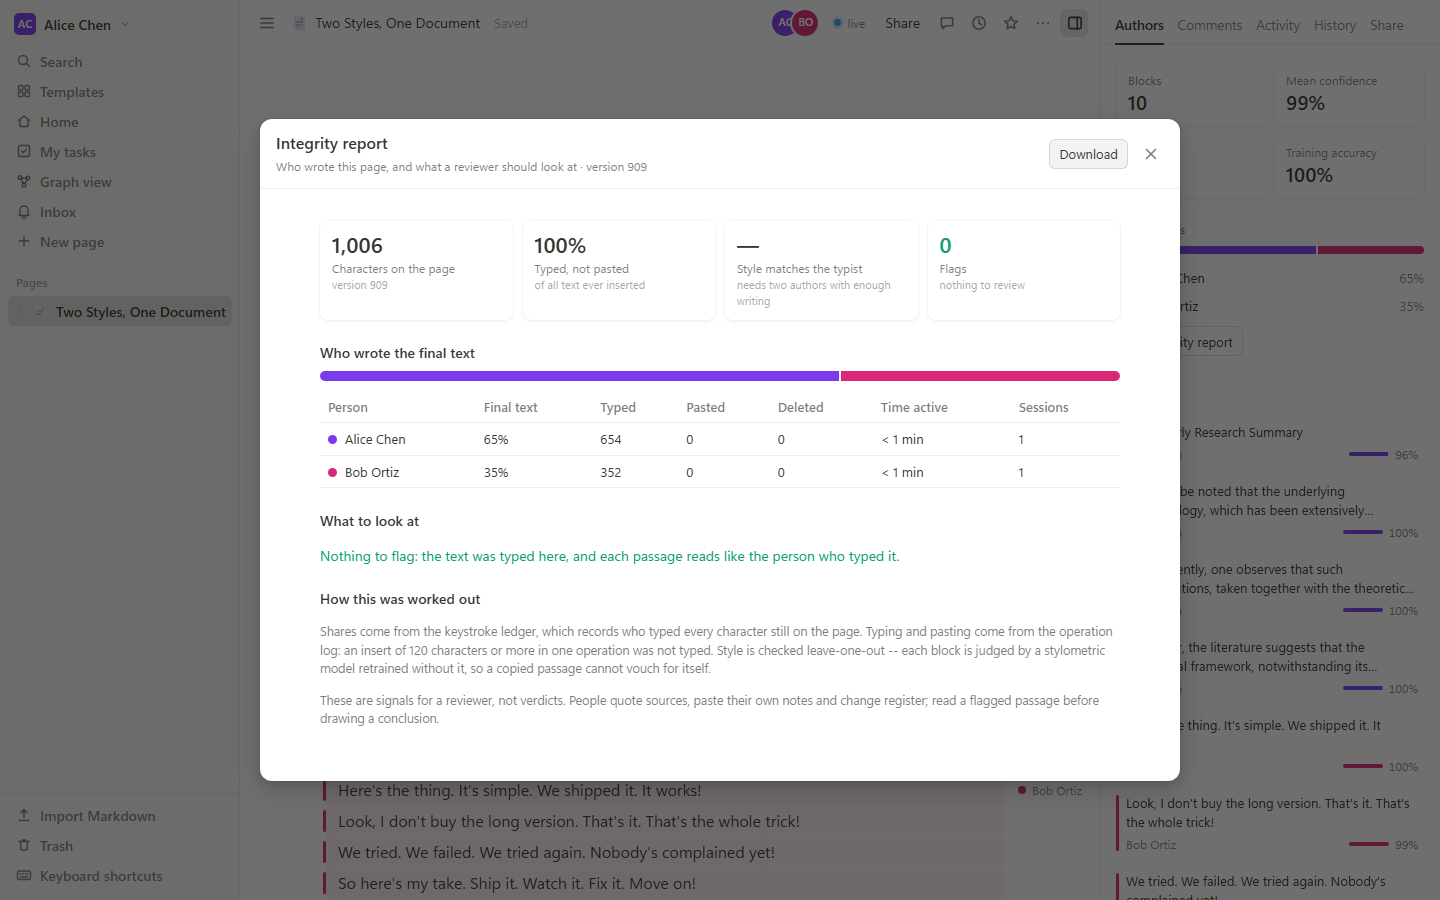
\includegraphics[width=\columnwidth]{fig/12-integrity.png}
\caption{Integrity report: per-person share and effort, pastes and style-mismatch flags.}
\label{fig:integrity}
\end{figure}

%--------------------------------------------------------------------
\section{Limitations}
Rich text is markup over a plain-text buffer, so formatting is a rendering concern and cannot span lines; styled-range OT or a CRDT is the upgrade path. Comments anchor by quoted text and lose their place if it is rewritten. Attribution needs writing to learn from, and style evidence between close collaborators is weak. Each document is pinned to one pod, so a pod failure moves its documents and editors should reload; a per-document lease, or a consensus-backed store such as one built on Raft~\cite{raft}, would remove this; the distributed-systems trade-offs involved are surveyed in~\cite{ddia}. The operation log grows without compaction. The measurements above come from a single machine and synthetic text, and a study with real collaborators is needed before attribution confidence can be treated as calibrated.

%--------------------------------------------------------------------
\section{Conclusion}
CollabDoc shows that a server-arbitrated OT engine and an authorship model can share one source of truth: the operation log that makes editing convergent also supplies the labels, evidence and history that attribution needs. The design yields low acknowledgement latency, an explicit abstention rule, and an integrity report that corrects a failure specific to stylometry on shared text, namely that copied passages vouch for themselves. Future work includes real-user evaluation, styled-range synchronisation, log compaction, and per-document leases for fail-over.

%--------------------------------------------------------------------
\section*{Project Links}
\noindent\textbf{Project demo:} [demo URL; the AWS stack is started and stopped on demand]\\
\textbf{GitHub repository:} N.~Kumar and B.~N., ``CollabDoc: a real-time collaborative document editor with operational transformation and stylometric authorship attribution,'' \url{https://github.com/Zerko-sd/CollabDoc}.\\
\textbf{Word-format copy of this paper:} [link, if provided].

\section*{Acknowledgment}
The authors thank the faculty and reviewers whose feedback shaped this work.

%--------------------------------------------------------------------
\begin{thebibliography}{99}
\bibitem{ellis1989} C.~A. Ellis and S.~J. Gibbs, ``Concurrency control in groupware systems,'' in \emph{Proc. ACM SIGMOD}, 1989, pp.~399--407. doi:10.1145/67544.66963. \url{https://doi.org/10.1145/67544.66963}
\bibitem{sun1998} C.~Sun, X.~Jia, Y.~Zhang, Y.~Yang, and D.~Chen, ``Achieving convergence, causality preservation, and intention preservation in real-time cooperative editing systems,'' \emph{ACM Trans. Comput.-Hum. Interact.}, vol.~5, no.~1, pp.~63--108, 1998. \url{https://doi.org/10.1145/274444.274447}
\bibitem{sun1998ot} C.~Sun and C.~Ellis, ``Operational transformation in real-time group editors: issues, algorithms, and achievements,'' in \emph{Proc. ACM CSCW}, 1998, pp.~59--68. \url{https://doi.org/10.1145/289444.289469}
\bibitem{nichols1995} D.~A. Nichols, P.~Curtis, M.~Dixon, and J.~Lamping, ``High-latency, low-bandwidth windowing in the Jupiter collaboration system,'' in \emph{Proc. ACM UIST}, 1995, pp.~111--120. \url{https://doi.org/10.1145/215585.215706}
\bibitem{ressel1996} M.~Ressel, D.~Nitsche-Ruhland, and R.~Gunzenh\"auser, ``An integrating, transformation-oriented approach to concurrency control and undo in group editors,'' in \emph{Proc. ACM CSCW}, 1996, pp.~288--297. \url{https://doi.org/10.1145/240080.240305}
\bibitem{oster2006} G.~Oster, P.~Urso, P.~Molli, and A.~Imine, ``Data consistency for P2P collaborative editing,'' in \emph{Proc. ACM CSCW}, 2006, pp.~259--268. \url{https://doi.org/10.1145/1180875.1180916}
\bibitem{shapiro2011} M.~Shapiro, N.~Pregui\c{c}a, C.~Baquero, and M.~Zawirski, ``Conflict-free replicated data types,'' in \emph{Proc. SSS}, LNCS vol.~6976, 2011, pp.~386--400. \url{https://doi.org/10.1007/978-3-642-24550-3_29}
\bibitem{kleppmann2017} M.~Kleppmann and A.~R. Beresford, ``A conflict-free replicated JSON datatype,'' \emph{IEEE Trans. Parallel Distrib. Syst.}, vol.~28, no.~10, pp.~2733--2746, 2017. \url{https://doi.org/10.1109/TPDS.2017.2697382}
\bibitem{weiss2009} S.~Weiss, P.~Urso, and P.~Molli, ``Logoot: a scalable optimistic replication algorithm for collaborative editing on P2P networks,'' in \emph{Proc. IEEE ICDCS}, 2009, pp.~404--412. \url{https://doi.org/10.1109/ICDCS.2009.75}
\bibitem{roh2011} H.-G. Roh, M.~Jeon, J.-S. Kim, and J.~Lee, ``Replicated abstract data types: building blocks for collaborative applications,'' \emph{J. Parallel Distrib. Comput.}, vol.~71, no.~3, pp.~354--368, 2011. \url{https://doi.org/10.1016/j.jpdc.2010.12.006}
\bibitem{nicolaescu2016} P.~Nicolaescu, K.~Jahns, M.~Derntl, and R.~Klamma, ``Near real-time peer-to-peer shared editing on extensible data types,'' in \emph{Proc. ACM GROUP}, 2016, pp.~39--49. \url{https://doi.org/10.1145/2957276.2957310}
\bibitem{kleppmann2019} M.~Kleppmann, A.~Wiggins, P.~van Hardenberg, and M.~McGranaghan, ``Local-first software: you own your data, in spite of the cloud,'' in \emph{Proc. ACM Onward!}, 2019, pp.~154--178. \url{https://doi.org/10.1145/3359591.3359737}
\bibitem{attiya2016} H.~Attiya, S.~Burckhardt, A.~Gotsman, A.~Morrison, H.~Yang, and M.~Zawirski, ``Specification and complexity of collaborative text editing,'' in \emph{Proc. ACM PODC}, 2016, pp.~259--268. \url{https://doi.org/10.1145/2933057.2933090}
\bibitem{fraser2009} N.~Fraser, ``Differential synchronization,'' in \emph{Proc. ACM DocEng}, 2009. \url{https://neil.fraser.name/writing/sync/}
\bibitem{mosteller1963} F.~Mosteller and D.~L. Wallace, ``Inference in an authorship problem,'' \emph{J. Amer. Statist. Assoc.}, vol.~58, no.~302, pp.~275--309, 1963. \url{https://doi.org/10.1080/01621459.1963.10500849}
\bibitem{stamatatos2009} E.~Stamatatos, ``A survey of modern authorship attribution methods,'' \emph{J. Amer. Soc. Inf. Sci. Technol.}, vol.~60, no.~3, pp.~538--556, 2009. \url{https://doi.org/10.1002/asi.21001}
\bibitem{koppel2009} M.~Koppel, J.~Schler, and S.~Argamon, ``Computational methods in authorship attribution,'' \emph{J. Amer. Soc. Inf. Sci. Technol.}, vol.~60, no.~1, pp.~9--26, 2009. \url{https://doi.org/10.1002/asi.20961}
\bibitem{juola2006} P.~Juola, ``Authorship attribution,'' \emph{Found. Trends Inf. Retr.}, vol.~1, no.~3, pp.~233--334, 2006. \url{https://doi.org/10.1561/1500000005}
\bibitem{burrows2002} J.~Burrows, ```Delta': a measure of stylistic difference and a guide to likely authorship,'' \emph{Lit. Linguist. Comput.}, vol.~17, no.~3, pp.~267--287, 2002. \url{https://doi.org/10.1093/llc/17.3.267}
\bibitem{evert2017} S.~Evert \emph{et al.}, ``Understanding and explaining Delta measures for authorship attribution,'' \emph{Digit. Scholarsh. Humanit.}, vol.~32, suppl.~2, pp.~ii4--ii16, 2017. \url{https://doi.org/10.1093/llc/fqx023}
\bibitem{narayanan2012} A.~Narayanan \emph{et al.}, ``On the feasibility of internet-scale author identification,'' in \emph{Proc. IEEE Symp. Security and Privacy}, 2012, pp.~300--314. \url{https://doi.org/10.1109/SP.2012.46}
\bibitem{monrose2000} F.~Monrose and A.~D. Rubin, ``Keystroke dynamics as a biometric for authentication,'' \emph{Future Gener. Comput. Syst.}, vol.~16, no.~4, pp.~351--359, 2000. \url{https://doi.org/10.1016/S0167-739X(99)00059-X}
\bibitem{killourhy2009} K.~S. Killourhy and R.~A. Maxion, ``Comparing anomaly-detection algorithms for keystroke dynamics,'' in \emph{Proc. IEEE/IFIP DSN}, 2009, pp.~125--134. \url{https://doi.org/10.1109/DSN.2009.5270346}
\bibitem{banerjee2012} S.~P. Banerjee and D.~L. Woodard, ``Biometric authentication and identification using keystroke dynamics: a survey,'' \emph{J. Pattern Recognit. Res.}, vol.~7, no.~1, pp.~116--139, 2012. \url{https://doi.org/10.13176/11.427}
\bibitem{lamport1978} L.~Lamport, ``Time, clocks, and the ordering of events in a distributed system,'' \emph{Commun. ACM}, vol.~21, no.~7, pp.~558--565, 1978. \url{https://doi.org/10.1145/359545.359563}
\bibitem{gilbert2002} S.~Gilbert and N.~Lynch, ``Brewer's conjecture and the feasibility of consistent, available, partition-tolerant web services,'' \emph{ACM SIGACT News}, vol.~33, no.~2, pp.~51--59, 2002. \url{https://doi.org/10.1145/564585.564601}
\bibitem{brewer2000} E.~A. Brewer, ``Towards robust distributed systems,'' keynote, ACM PODC, 2000. \url{https://people.eecs.berkeley.edu/~brewer/cs262b-2004/PODC-keynote.pdf}
\bibitem{karger1997} D.~Karger \emph{et al.}, ``Consistent hashing and random trees,'' in \emph{Proc. ACM STOC}, 1997, pp.~654--663. \url{https://doi.org/10.1145/258533.258660}
\bibitem{thaler1998} D.~G. Thaler and C.~V. Ravishankar, ``Using name-based mappings to increase hit rates,'' \emph{IEEE/ACM Trans. Netw.}, vol.~6, no.~1, pp.~1--14, 1998. \url{https://doi.org/10.1109/90.663936}
\bibitem{rfc6455} I.~Fette and A.~Melnikov, ``The WebSocket protocol,'' RFC 6455, IETF, 2011. \url{https://doi.org/10.17487/RFC6455}
\bibitem{kreps2011} J.~Kreps, N.~Narkhede, and J.~Rao, ``Kafka: a distributed messaging system for log processing,'' in \emph{Proc. NetDB}, 2011. \url{https://www.microsoft.com/en-us/research/wp-content/uploads/2017/09/Kafka.pdf}
\bibitem{burns2016} B.~Burns, B.~Grant, D.~Oppenheimer, E.~Brewer, and J.~Wilkes, ``Borg, Omega, and Kubernetes,'' \emph{Commun. ACM}, vol.~59, no.~5, pp.~50--57, 2016. \url{https://doi.org/10.1145/2890784}
\bibitem{rfc8018} K.~Moriarty, B.~Kaliski, and A.~Rusch, ``PKCS \#5: password-based cryptography specification version 2.1,'' RFC 8018, IETF, 2017. \url{https://doi.org/10.17487/RFC8018}
\bibitem{rfc7519} M.~Jones, J.~Bradley, and N.~Sakimura, ``JSON Web Token (JWT),'' RFC 7519, IETF, 2015. \url{https://doi.org/10.17487/RFC7519}
\bibitem{sklearn} F.~Pedregosa \emph{et al.}, ``Scikit-learn: machine learning in Python,'' \emph{J. Mach. Learn. Res.}, vol.~12, pp.~2825--2830, 2011. \url{https://jmlr.org/papers/v12/pedregosa11a.html}
\bibitem{fastapi} S.~Ram\'irez, ``FastAPI documentation.'' \url{https://fastapi.tiangolo.com}
\bibitem{ddia} M.~Kleppmann, \emph{Designing Data-Intensive Applications}. O'Reilly Media, 2017. \url{https://dataintensive.net}
\bibitem{raft} D.~Ongaro and J.~Ousterhout, ``In search of an understandable consensus algorithm,'' in \emph{Proc. USENIX ATC}, 2014, pp.~305--319. \url{https://www.usenix.org/conference/atc14/technical-sessions/presentation/ongaro}
\end{thebibliography}

\end{document}
